\section{Sliding Mode Design Figures}\label{slidingModeDesignFigures}
\vspace{-.2cm}
\begin{adjustwidth}{-1.1cm}{-1.1cm}
  \begin{minipage}{\textwidth}
    \begin{minipage}{0.58\textwidth}
      \begin{figure}[H]
        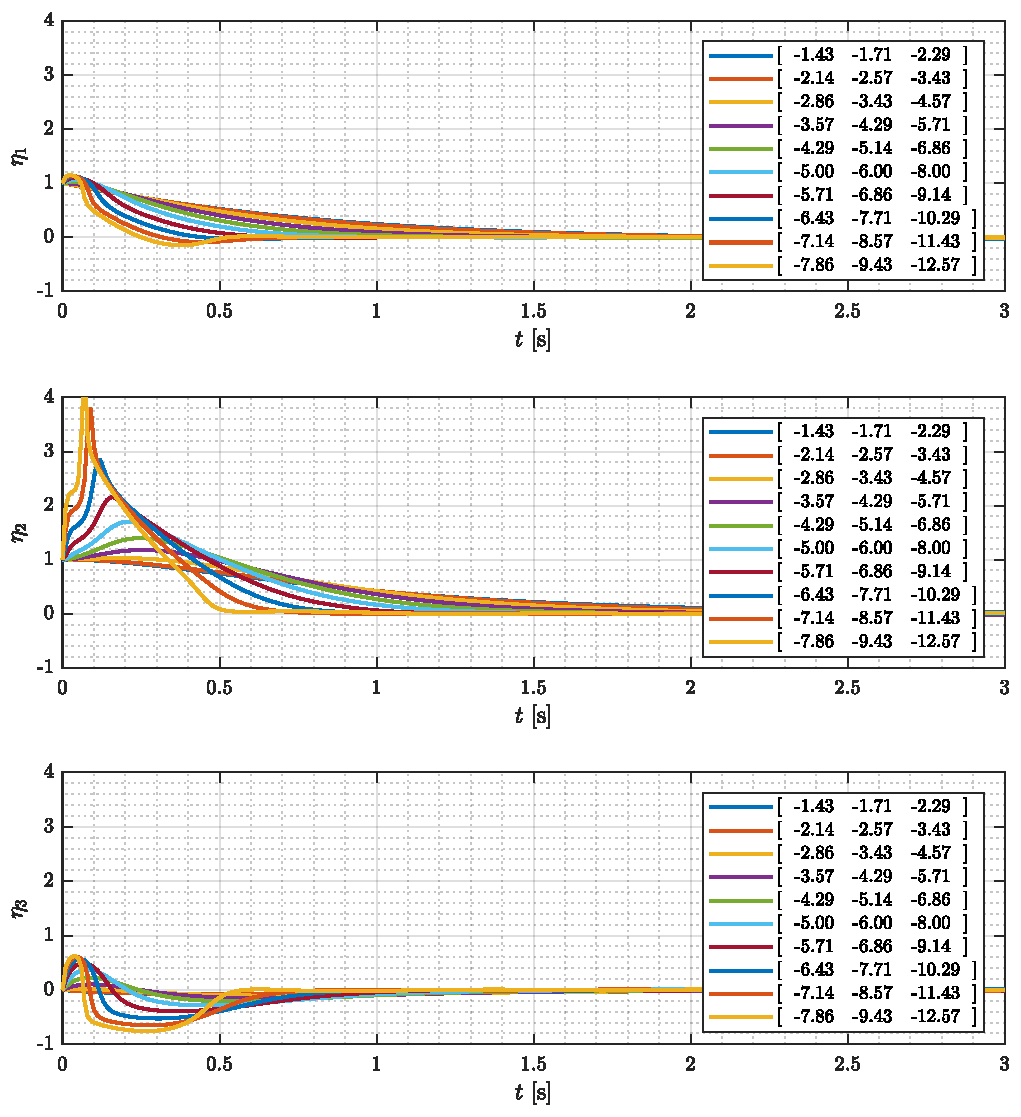
\includegraphics[width=\textwidth]{figures/reducedOrderControlMany}
        \caption{Comparison of some different choices of pole placements for the reduced order system. The chosen pole placement is [ $-5\ $ $-6\ $ $-9$ ] resulting in \\ $\vec{k} =$ [ $-27.50\ $ $13.34\ $ $29.30$ ].}
        \label{fig:reducedOrderControlMany}
      \end{figure}
    \end{minipage}
    \begin{minipage}{0.58\textwidth}
      \begin{figure}[H]
        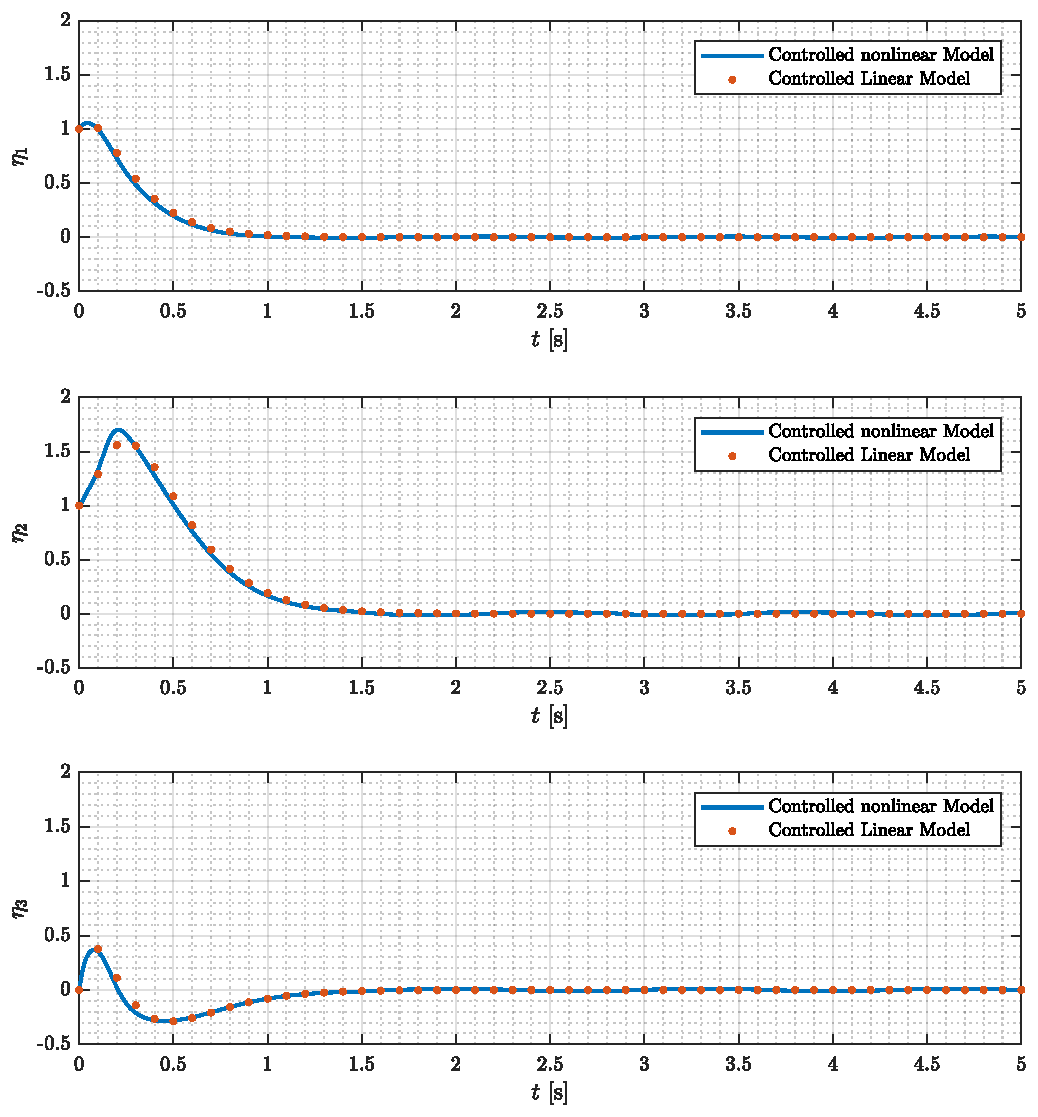
\includegraphics[width=\textwidth]{figures/reducedOrderControl}
        \caption{Result of the chosen pole placement for the reduced order system with comparison between linearized and non-linear plant using lsim and ode45 respectively.\\ \vspace{14pt}}
        \label{fig:reducedOrderControl}
      \end{figure}
    \end{minipage}
  \end{minipage}
\end{adjustwidth}
\vspace{.5cm}

\begin{figure}[H]
  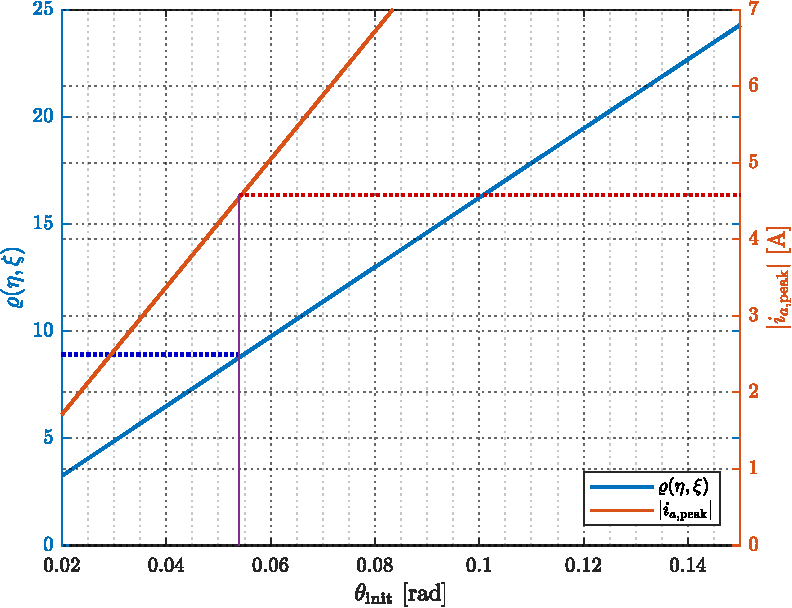
\includegraphics[width=.6\textwidth]{figures/chooseRho}
  \caption{$\dot{\theta}=0$ and the horizontal line marks $\theta_\mathrm{max} =$ \SI{0.0540}{rad} dictated by the current limitation of the motor, $i_{a,\mathrm{max}} = \SI{4.58}{A}$, and thereby indicating the maximum gain, $\varrho(\vec{\eta},\xi) = 8.9095$, with $\beta_0=0.1$, allowing some margin for the supposed operational region.}
  \label{fig:chooseRho}
\end{figure}